\chapter{Soft Actor-Critic}


待重读的资源:
\begin{itemize}
%\setlength{\itemsep}{0pt}
%\setlength{\parsep}{0pt}
\setlength{\parskip}{0pt}
\item[-]
\url{https://blog.csdn.net/weixin_44436360/article/details/108077422}

\item[-]
\url{https://www.pair.toronto.edu/csc2621-w20/assets/slides/lec4_sac.pdf}

\item[-]
\url{https://blog.csdn.net/weixin_44044411/article/details/119922423}

\item[-]
\url{https://www.ics.uci.edu/~dechter/courses/ics-295/winter-2018/papers/nips/soft-actor-critic-nips-2017.pdf}

\item[-]
\url{https://zhuanlan.zhihu.com/p/70360272}
\end{itemize}

\section{Overview}


\subsection{Actor-critic algorithm}
% https://greentec.github.io/reinforcement-learning-fourth-en/

Actor Critic 合并了以值为基础(比如$Q$-learning)和以动作概率为基础(比如 Policy 
Gradients)的两类强化学习算法。Actor 的前身是 Policy Gradients, 
该方法可以在连续动作中选取合适的动作;Critic 的前生是 $Q$-learning 
或者其他以值为基础的学习法, 能进行单步更新, 但并不能处理连续动作。而传统的 Policy 
Gradients 则是回合更新。我们就比较贪心了,又想处理连续动作,又想单步更新,
那就你们两个结合一下呗。actor 网络输入 state,输出action;critic 网络输入为 state
和 action,输出为 $Q$ 值,就组成了 Actor Critic。但传统 Actor-Critic 
前后相关性高,学习片面,于是人们有学习了 DQN 中的方法,使用一个 Replay buffer 
和两个结构相同, 但参数更新频率不同的神经网络来训练,于是就有了 DDPG。

Here we give a brief introduction to actor-critic algorithms that 
outperform many algorithms in applications.

The Dueling DQN was the idea of ​​dividing the network results into $V$ and 
$A$ before reassembling them before we got the $Q$ value. Similar, but 
different Actor-Critic algorithm use two networks: an Actor network and 
a Critic network.

The Actor determines the action when the state is given, and Critic 
evaluates the value of the state. Actor-critic is quite similar to 
Dueling DQN, but the Dueling DQN is the sum of the two values to get the 
$Q$ value and the Actor-Critic does not combine the values at the end. 
Depending on the implementation, the decoders of the receiving network 
may join together, but the structure of the Dueling DQN and the 
Actor-Critic will differ depending on whether the $Q$ values are combined 
or not. Of course, there is a difference between using DQN in Replay 
Buffer and not using Actor-Critic.

\begin{figure}[h]
\centering
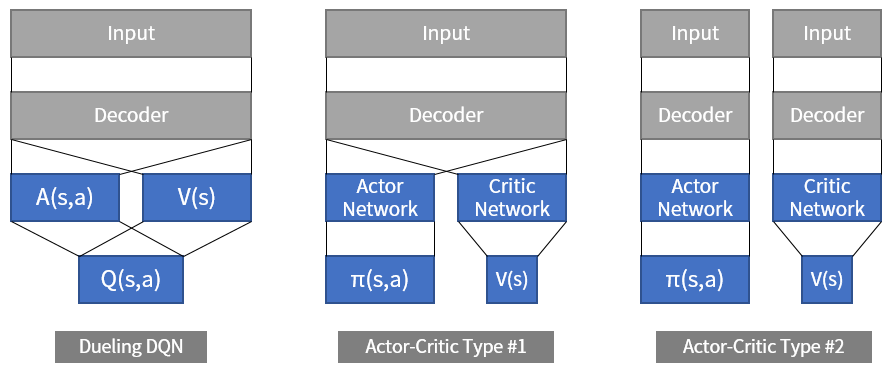
\includegraphics[scale=0.618]{pix/sac/rl4_0.png}
\caption{The structure of the actor-critic algorithm can be divided into 
two types depending on whether or not parameter sharing is applied to 
the decoders that interpret the input.}
\label{fig:two_types_actor_critic}
\end{figure}

The biggest difference between DQN and Actor-Critic is whether to use 
Replay Buffer. Unlike DQN, Actor-Critic does not use Replay Buffer but 
learns the model using state($s$), action($a$), reward($r$), and next 
state($s'$) obtained at every step.

DQN obtains the value of $Q(s,a)$ and actor-critic obtains the value of 
$\pi(s,a)$ and $V(s)$. $V(s)$ is the value function we've covered so 
far, and $\pi(s,a)$ is the probability of taking a specific action in 
some state. Usually this probability can be obtained using softmax. 
Softmax calculates certain values by exponentiation with $e$ as the base, 
then sums and divides to convert the sum to a probability of $1.0$.
$$
P(z)=\frac{e^{z_j}}{\sum^K_{k=1}e^{z_k}} 
\qquad (\text{for} \quad j=1, \ldots, K)
$$
For example, if we have a value of $[2,1,0]$ and convert it to softmax,
\begin{eqnarray*}
sum &=& \sum^K_{k=1} e^{z_k} \\
&=& e^2 + e^1 + e^0 \\
&=& 11.1073 \notag\\
\\
softmax &=& \frac{e^{z_j}}{\sum^K_{k=1} e^{z_k}} \\
&=& \left[\frac{e^2}{sum}, \frac{e^1}{sum}, \frac{e^0}{sum}\right] \\
&=& [0.67, 0.24, 0.09] \notag
\end{eqnarray}

It is a probability value of $[0.67, 0.24, 0.09]$. Softmax function is 
used in many areas of deep learning, such as image classification or 
text generation. Reinforcement learning can also be used to obtain the 
action probability of an agent.

The method of directly learning the behavior probability of an agent 
is called REINFORCE or policy gradient. A policy is a policy about what 
action the agent will take, and a gradient means that the policy value 
is updated through differentiation and the optimal policy is searched. 
However, since the method of directly learning the action probability 
of the agent is unstable, it is the core of the Actor-Critic to increase 
the stability by using the value function together.

\begin{figure}[h]
\centering
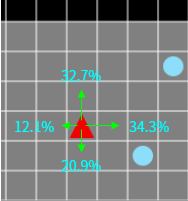
\includegraphics[scale=0.8]{pix/sac/rl4_6.png}
\caption{The policy value directly represents the probability that each 
action($a$) will occur in any state($s$).}
%\label{fig:label}
\end{figure}

Using the Advantage as the expected output of Actor-Critic's Actor will 
be {\bf A}dvantage {\bf A}ctor-{\bf C}ritic, {\bf A}2{\bf C}. Advantage 
is a value that determines how much better than expected ($V(s)$). 
Advantage generally uses the value obtained by subtracting $V(s)$ from 
$Q(s,a)$.
$$
A(s,a) = Q(s,a) - V(s)
$$

However, $Q(s,a)$ is not shown in the structure of the Actor-Critic 
algorithm in Figure \ref{fig:two_types_actor_critic}. But as we know,
$$
\text{Actual\_Value} \simeq \text{Present\_Value} + \text{Future\_Value}
$$
The present value is reward, and the future value is replaced with the 
value function $V(s′)$ of the next state, the following expression can 
be obtained.
$$
Q(s,a) \simeq R + \gamma V(s')
$$
In summary, the formula for obtaining Advantage changes as follows.
$$
A(s,a) \simeq R + \gamma V(s') - V(s)
$$
The $V(s)$ value calculated by the Critic Network will also affect the 
calculation of the Actor Network.

The most famous example affected by the Actor-Critic algorithm is the 
Deep Mind's AlphaGo. They learned the policy network corresponding to 
the actor and the value network corresponding to the critic so that they 
could find the optimal action in the given environment.

\begin{figure}[h]
\centering
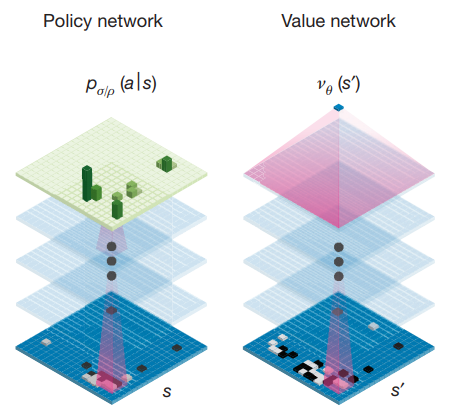
\includegraphics[scale=0.618]{pix/sac/rl4_1.png}
\caption{Deep Mind's AlphaGo learned agents through two networks: 
Policy Network and Value Network.}
%\label{fig:label}
\end{figure}

We can not create an AlphaGo at once, but we can train an agent with 
greatly improved action with the Actor-Critic algorithm in Grid World.

\begin{figure}[h]
\centering
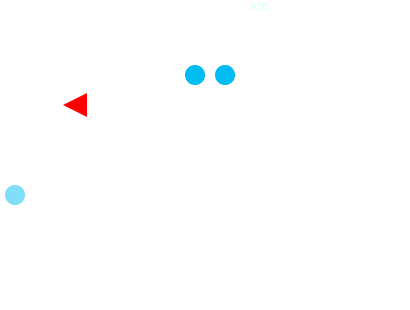
\includegraphics[scale=0.618]{pix/sac/download.png}
\caption{Learn(Actor-Critic)Run(Actor-Critic)}
%\label{fig:label}
\end{figure}

From about 100 episodes, the agent starts to look for the ball. Even 
if there is no ball in sight, the agent gets closer to the ball through 
navigation, and if there are multiple balls in sight, it almost reaches 
all the balls without missing.

How do these agents move? In Unity, we will look at ideas from Arthur 
Juliani’s blog article on ML-Agent, a reinforcement learning agent, to 
see how A2C agents judge the environment.

% https://greentec.github.io/reinforcement-learning-fourth-en/
% https://greentec.github.io/reinforcement-learning-fourth-en/#:~:text=The%20biggest%20difference%20between%20DQN%20and%20Actor-Critic%20that,and%20next%20state%20%28s%E2%80%99%29%20obtained%20at%20every%20step.
% to be continue


\subsection{Soft actor-critic}

% https://blog.csdn.net/weixin_44436360/article/details/108077422
% https://zhuanlan.zhihu.com/p/70360272

Soft actor-critic is based on the maximum entropy reinforcement learning 
framework, which considers the entropy augmented objective where and are 
the state and the action, and the expectation is taken over the policy and 
the true dynamics of the system.

Robot Learning正在快速的发展,其中深度强化学习deep reinforcement learning(DRL),
特别是面向连续控制continous control的DRL算法起着重要的作用。
在这一领域中,目前有三类行之有效的modle free DRL算法:
\begin{itemize}
%\setlength{\itemsep}{0pt}
%\setlength{\parsep}{0pt}
\setlength{\parskip}{0pt}
\item[-]
TRPO,PPO
\item[-]
DDPG及其拓展(D4PG,TD3等)
\item[-]
Soft Q-Learning, Soft Actor-Critic
\end{itemize}


PPO算法是主流的DRL算法,同时面向离散控制和连续控制,在OpenAI Five上取得了巨大成功。
但是PPO是一种on-policy算法,存在sample inefficiency的缺点,需要巨量的采样才能学习。
DDPG及其拓展是面向连续控制的off-policy的算法,相对于PPO来说更sample efficient,
但是它存在对其超参数敏感,收敛效果差的问题。DDPG训练的是一种确定性策略deterministic policy,
即每一个state下都只考虑最优的一个动作。DDPG的拓展版D4PG从paper中的结果看取得了非常好的效果,
但是并没有开源,目前github上也没有人能够完全复现Deepmind的效果。

SAC算法是面向最大熵强化学习开发的一种off-policy算法。
与DDPG相比,SAC使用的是随机策略,相比确定性策略具有一定的优势。
Soft Actor-Critic在公开的benchmark中取得了非常好的效果,并且能直接应用到真实机器人上。
最关键的是,Soft Actor-Critic是完全开源的,因此,深入理解Soft Actor-Critic 算法具有非常重要的意义。

\subsection{相关链接}

Papers:
\begin{itemize}
%\setlength{\itemsep}{0pt}
%\setlength{\parsep}{0pt}
\setlength{\parskip}{0pt}
\item[-]
\href{https://arxiv.org/abs/1801.01290}{Soft Actor-Critic: 
Off-Policy Maximum Entropy Deep Reinforcement Learning with a Stochastic Actor}
\item[-]
\href{https://arxiv.org/abs/1812.05905}{Soft Actor-Critic Algorithms and Applications}
\item[-]
\href{https://arxiv.org/abs/1702.08165}{Reinforcement Learning with Deep Energy-Based Policies (Soft Q-Learning)}
\end{itemize}

Codes:
\begin{itemize}
%\setlength{\itemsep}{0pt}
%\setlength{\parsep}{0pt}
\setlength{\parskip}{0pt}
\item[-]
\href{https://github.com/rail-berkeley/softlearning}{rail-berkeley/softlearning (原作者实现)}
\item[-]
\href{https://github.com/vitchyr/rlkit}{vitchyr/rlkit}
\item[-]
\href{https://github.com/openai/spinningup}{openai/spinningup}
\item[-]
\href{https://github.com/hill-a/stable-baselines}{hill-a/stable-baselines}
\end{itemize}


\section{SAC}

% \noindent 最大熵强化学习算法SAC \\
% https://www.toutiao.com/article/6845540775015481870/
% https://bair.berkeley.edu/blog/2018/12/14/sac/


SAC:Soft Actor-Critic,Off-Policy Maximum Entropy Deep Reinforcement 
Learning with a Stochastic Actor。

Soft actor-critic is based on the maximum entropy reinforcement learning 
framework, which considers the entropy augmented objective

\begin{equation}\label{sac_entropy_augmented_objective}
J(\pi) = \mathbb{E}_\pi\left[
\sum_tr(s_t, a_t) - \alpha \log\left(\pi(a_t | s_t)\right)
\right],
\end{equation}
\noindent{}where $s_t$ and $a_t$ are the state and the action, and the 
expectation is taken over the policy and the true dynamics of the system. 
In other words, the optimal policy not only maximizes the expected return 
(first summand) but also the expected entropy of itself (second summand). 
The trade-off between the two is controlled by the non-negative temperature 
parameter $\alpha$, and we can always recover the conventional, maximum 
expected return objective by setting $\alpha=0$. We can view this objective 
as an entropy constrained maximization of the expected return, and learn 
the temperature parameter automatically instead of treating it as a 
hyperparameter. 
\url{https://arxiv.org/abs/1812.05905}

This objective can be interpreted in several ways. We can view the entropy 
term as an uninformative (uniform) prior over the policy, but we can also 
view it as a regularizer or as an attempt to trade off between exploration 
(maximize entropy) and exploitation (maximize return). In 
\href{https://bair.berkeley.edu/blog/2017/10/06/soft-q-learning/}{another post}, 
the Berkeley group gave a broader overview and proposed applications that are 
unique to maximum entropy RL, and a probabilistic view of the objective is 
discussed in a \href{https://arxiv.org/abs/1805.00909}{tutorial}. 
Soft actor-critic maximizes this objective by parameterizing a Gaussian policy 
and a $Q$-function with a neural network, and optimizing them using approximate 
dynamic programming. They defer further details of soft actor-critic to the 
\href{https://arxiv.org/abs/1812.05905}{technical report}. In this section, 
we will view the objective as a grounded way to derive better reinforcement 
learning algorithms that perform consistently and are sample efficient enough 
to be applicable to real-world robotic applications, and—perhaps surprisingly—can 
yield state-of-the-art performance under the conventional, maximum expected 
return objective (without entropy regularization) in simulated benchmarks.


\subsection{模型结构}

模型同时学习action value Q、state value V和policy $\pi$。

V中引入Target V,供Q学习时使用;Target Network使学习有章可循、效率更高。

Q有两个单独的网络,选取最小值供V和$\pi$学习时使用,希望{\bf 减弱$Q$的过高估计}。

$\pi$学习的是分布的参数:均值和标准差;这与DDPG不同,DDPG的$\pi$是Deterministic的,
输出直接就是action,而{\bf SAC学习的是个分布},学习时action需要从分布中采样,
是{\bf Stochastic}的。

\begin{figure}[h]
\centering
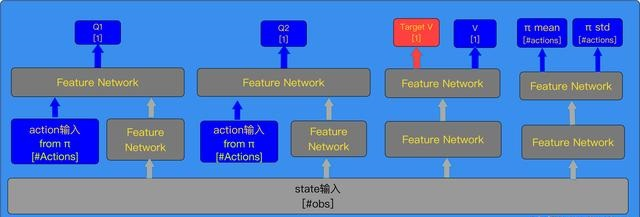
\includegraphics[scale=0.7]{pix/sac.jpg}
\caption{SAC}
%\label{fig:label}
\end{figure}


\subsection{Soft}

Soft,Smoothing,Stable。

原始的强化学习的目标是最大化累计reward:
\begin{equation}\label{rl_objective_function}
\sum_t\mathbb{E}_{(s_t,a_t)\sim\rho_\pi}\left[r(s_t, a_t)\right]
\end{equation}
其学习目标很直接,就是学习一个policy使得累加的reward期望值最大:
\begin{equation}\label{rl_reward_function}
\pi^* = \arg\max_\pi \mathbb{E}_{(s_t,a_t)\sim\rho_\pi}
\Big[ \sum_t r(s_t, a_t) \Big]
\end{equation}

\noindent 而强化学习最大熵目标函数(maximum entropy objective)则如下,比上面这个最初的累计奖赏,
增加了policy $\pi$的每一次输出的action的信息熵:

\begin{equation}\label{maximum_entropy_objective}
\pi^* = \arg\max_\pi \mathbb{E}_{(s_t,a_t)\sim\rho_\pi}
\Big[ \sum_t \big(
\underbrace{r(s_t, a_t)}_{\text{reward}} + 
\underbrace{\alpha \mathcal{H}(\pi(\cdot | s_t))}_{\text{entropy}}
\big)\Big]
\end{equation}
上式中的$\alpha$确定了熵项对于奖励的相对重要性。
与传统的DRL学习目标不同,不仅想要长期的回报最大,
还想要policy的每一次输出的action的熵最大。这样做其实就是为了让策略随机化,
即输出的每一个action的概率尽可能分散,而不是集中在一个action上。
也是在鼓励探索,为具有相似的$Q$值的动作分配近乎均等的概率,
不会给动作范围内任何一个动作分配非常高的概率,避免了反复选择同一个动作而陷入次优。
同时通过最大化奖赏,放弃明显没有前途的策略(放弃低奖赏策略)。
总的来说,具有以下几个优势:
\begin{itemize}
%\setlength{\itemsep}{0pt}
%\setlength{\parsep}{0pt}
\setlength{\parskip}{0pt}
\item[(1)]
更强的探索能力;
\item[(2)]
更鲁棒,面对干扰的时候能更容易做出调整;
\item[(3)]
训练速度加快(最大熵使探索更加均匀)。
\end{itemize}

A3C目标函数里的熵正则项和形式一样,只是作为正则项,系数很小。

\begin{equation}\label{SAC_entropy_of_policy}
J(\pi) = \sum_{t=0}^{T-1} \mathbb{E}_{(s_t,a_t)\sim\rho_\pi}
[r(s_t, a_t) + \alpha \mathcal{H}(\pi(\cdot | s_t))]
\end{equation}


\subsection{soft policy evaluation}

\cite{YZhang2020}
\parencite{YZhang2020}


对于一个固定的策略$\pi$, 在Soft Policy Iteration中,
近似{\bf soft $Q$-value}可以通过Bellman backup算子迭代出来,迭代更新规则如下:
\begin{equation}\label{soft_policy_evaluation}
\mathcal{T}^\pi Q(s_t, a_t) \triangleq r(s_t, a_t) 
+ \gamma \mathbb{E}_{s_{t+1}\sim\rho_s} [V^\pi(s_{t+1})],
\end{equation}
上式即是所谓的Bellman backup operator,作用范围为算子
$Q: \mathcal{S} \times \mathcal{A} \rightarrow \mathcal{R}$,
其中$V^\pi(s)$为soft state value function:
$$
V^\pi(s_t) = \mathbb{E}_{a_t\sim\pi}[Q^\pi(s_t,a_t)-\alpha\log\pi(a_t|s_t)].
$$
\begin{emp_box}
上式中的$\alpha$在大多数文献中并未出现,具体原因待查。
\end{emp_box}
If we define the entropy augmented reward as
$$
r_\pi(s_t,a_t) \triangleq r(s_t, a_t) 
+ \alpha\gamma \mathbb{E}_{s_{t+1}\sim\rho_s}
\left[ \mathcal{H}\left( \pi(\cdot | s_{t+1}) \right) \right]
$$
then we have
\begin{align*}
&\quad\ r(s_t, a_t) + \gamma \mathbb{E}_{s_{t+1}\sim\rho_s} 
[V^\pi(s_{t+1})] \\
&= r(s_t, a_t) + \gamma \mathbb{E}_{s_{t+1}\sim\rho_s}
\left[ 
\mathbb{E}_{a_{t+1}\sim\pi} 
\left[
Q^\pi(s_{t+1},a_{t+1}) - \alpha\log\pi(a_{t+1}|s_{t+1})
\right]
\right] \\
&= r(s_t, a_t) + \gamma \mathbb{E}_{s_{t+1}\sim\rho_s, a_{t+1}\sim\pi} 
\left[ Q^\pi(s_{t+1},a_{t+1}) \right] 
+ \alpha\gamma \mathbb{E}_{s_{t+1}\sim\rho_s} 
\left[ \mathcal{H}\left( \pi(\cdot | s_{t+1}) \right) \right] \\
&= r_\pi(s_t,a_t) + \gamma \mathbb{E}_{s_{t+1}\sim\rho_s, a_{t+1}\sim\pi} 
\left[ Q^\pi(s_{t+1},a_{t+1}) \right]. 
\end{align}
With the standard convergence results for policy evaluation, we could 
know that $Q^k$ will converge to the soft $Q$-value of $\pi$ as 
$k\rightarrow \infty$, with any $Q^0$ ($|\mathcal{A}| <\infty$) and 
$Q^{k+1} = \mathcal{T}^\pi Q^k$.

\begin{lemma}\label{lemma_soft_policy_evaluation}
(Soft Policy Evaluation). Consider the soft Bellman backup operator 
$\mathcal{T}^\pi$ in Equation (\ref{soft_policy_evaluation}) and a 
mapping $Q^0:\mathcal{S}\times\mathcal{A} \rightarrow \mathbb{R}$ 
with $|\mathbb{A}| < \infty$, and define $Q^{k+1} = \mathcal{T}^\pi Q^k$.
Then the sequence $Q^k$ will converge to the Soft Q-value of $\pi$ as 
$k\rightarrow \infty$.
\end{lemma}
这一引理说明soft policy evaluation可以通过$Q^{k+1} = \mathcal{T}^\pi Q^k$
进行迭代,若迭代无数次,最终会收敛到策略$\pi$的soft $Q$-value function.

根据{\bf 信息熵}的定义:
$$
H(U) = E[-\log p_i] = - \sum_{i=1}^n p_i\log p_i
$$
soft state value function和maximum entropy objective在形式上还是一致的。
系数$\alpha$能通过调节$Q$-value消除掉,可忽略。

TD3的soft state value function V形式与Soft Policy Iteration中类似,
但是SAC的action是通过对policy $\pi$采样确定地得到,
每条数据数据的信息熵就是其不确定性$-\log\pi(a|s)$;但考虑整个批量batch数据,
其整体还是$\pi$的信息熵,与maximum entropy方向一致。

信息熵越大,分布越均匀,所以最大化信息熵,有利于增加模型的探索能力。


\subsection{Soft State Value 目标函数}

通过$Q$和$\pi$网络近似$V$,注意$s$来自Experience Replay Buffer,
但是$a$来自当前的$\pi$。

\begin{figure}[h]
\centering
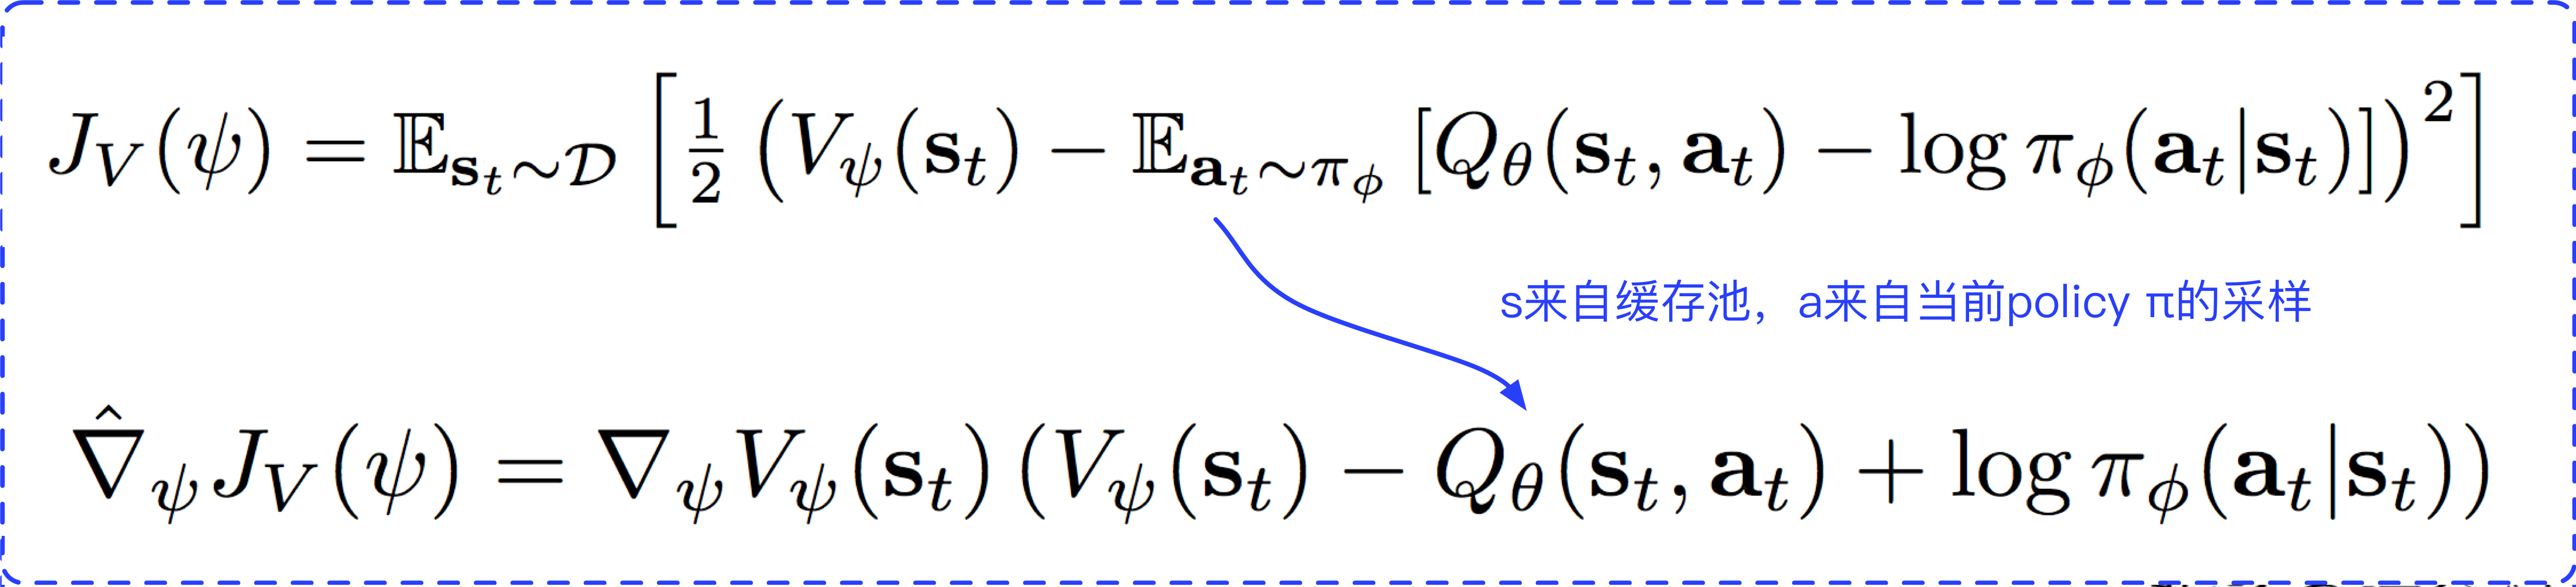
\includegraphics[scale=0.13]{pix/soft_state_value.png}
\caption{Soft state value}
%\label{fig:label}
\end{figure}


\subsection{Soft Q-Value 目标函数}

通过$V$近似$Q$,这里的$V$来自TargetNetwork $V$。
$r(s,a)$是环境的即时奖赏;$s_{t+1}$来自环境,由于环境是model-free,
可以理解成$s_{t+1}$是确定的。

\begin{figure}[h]
\centering
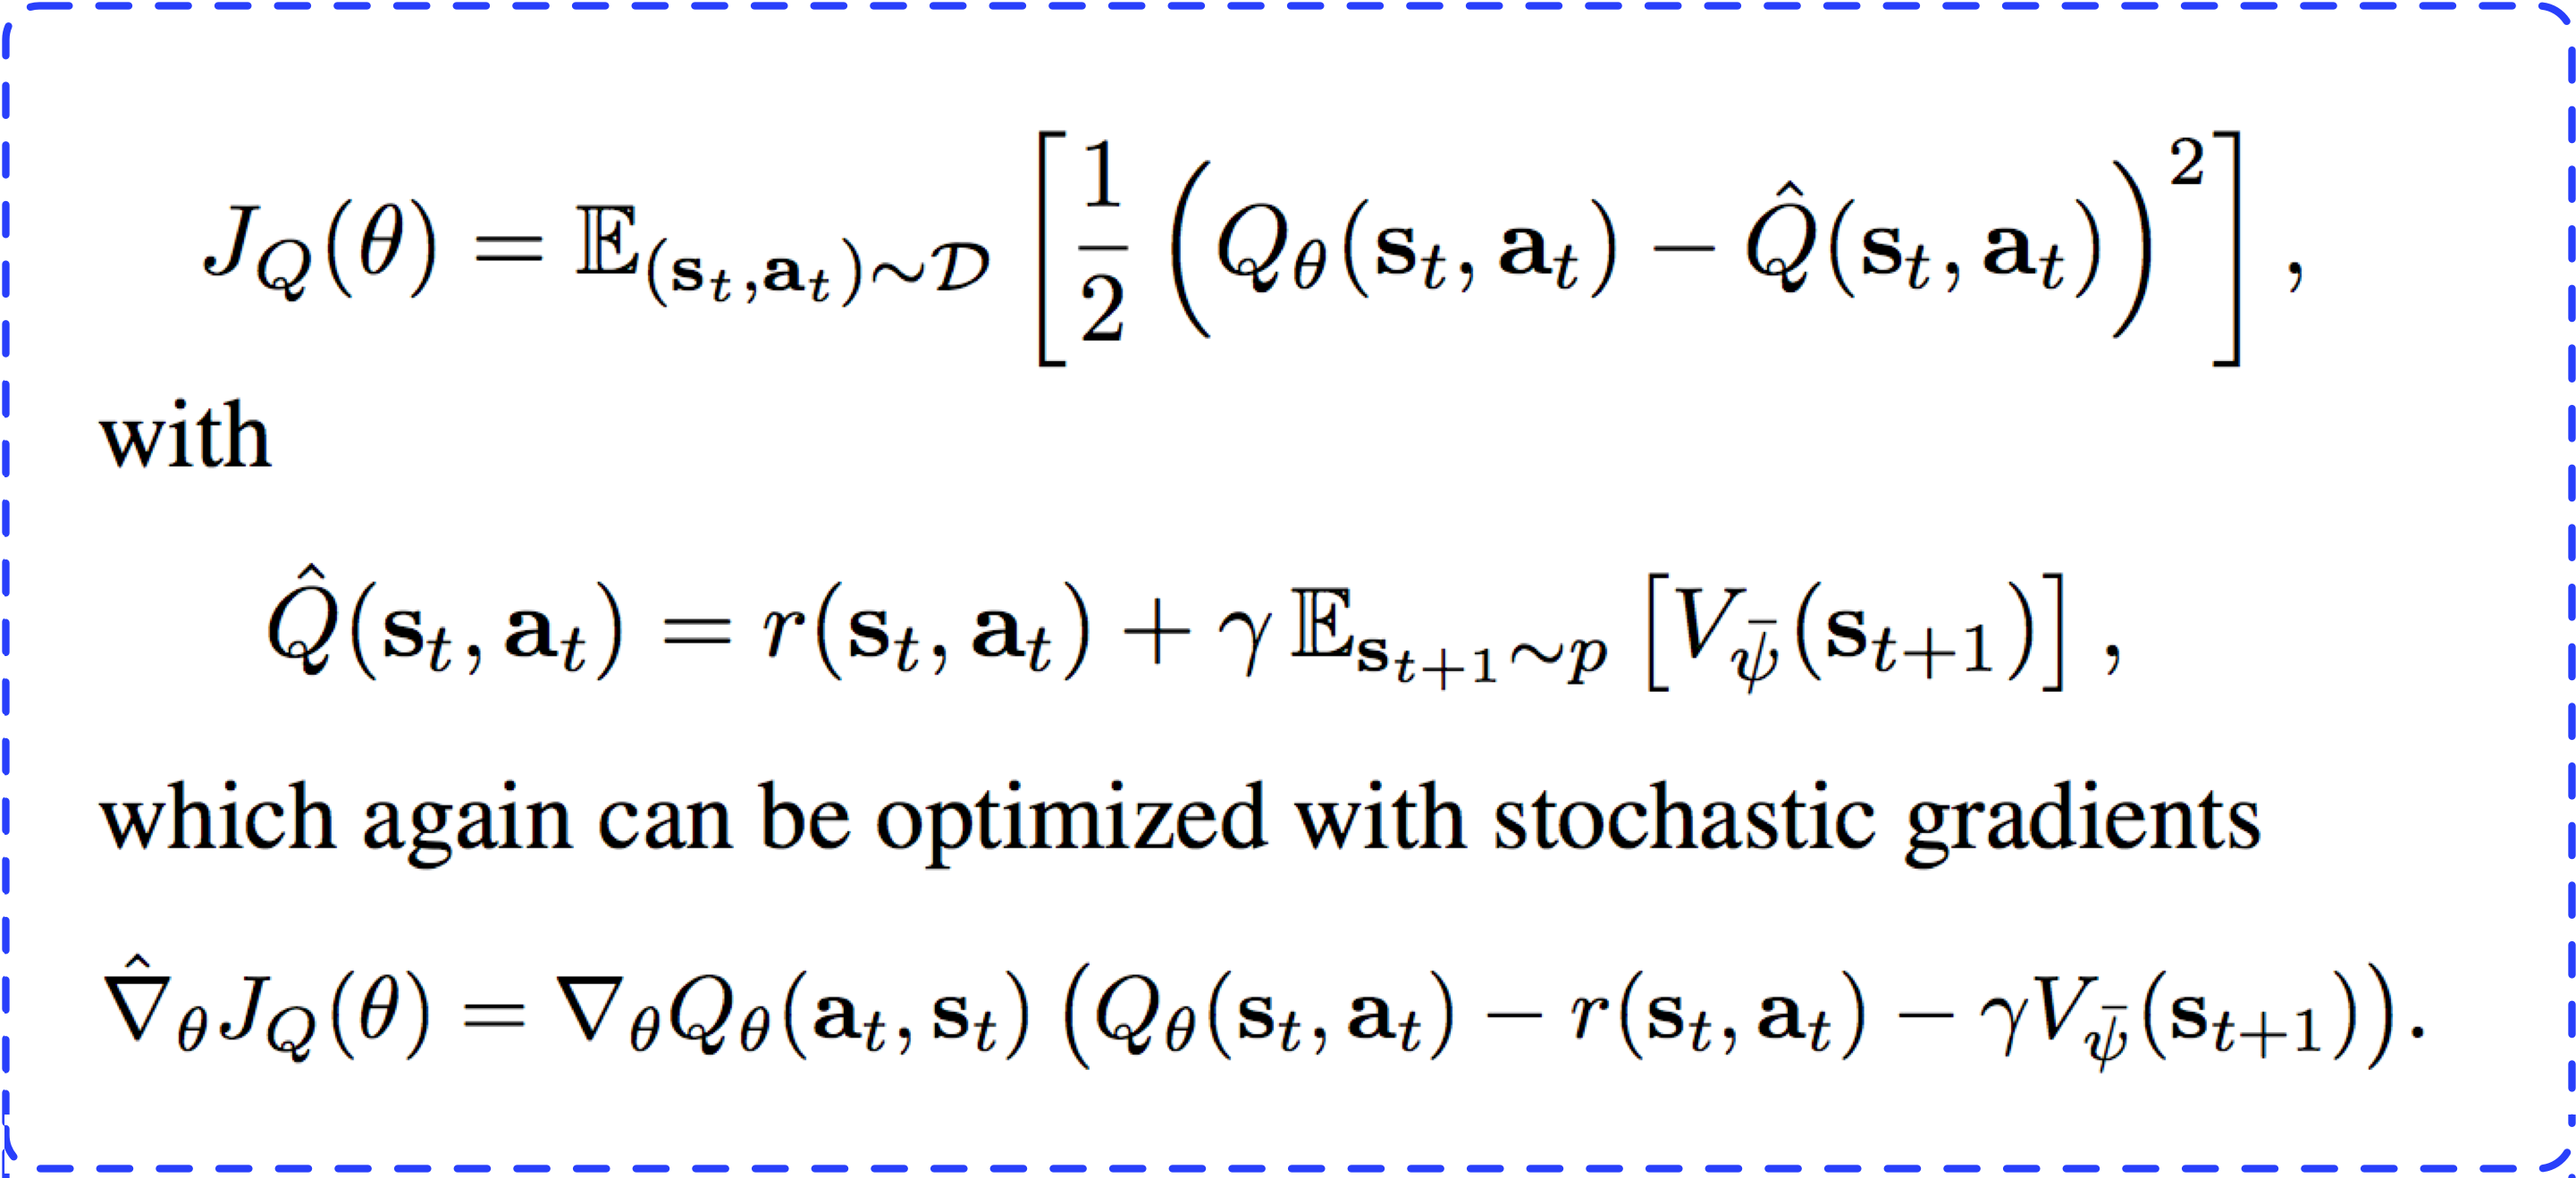
\includegraphics[scale=0.2]{pix/soft_q_value.png}
\caption{Soft Q value}
%\label{fig:label}
\end{figure}


\subsection{Policy 目标函数}

通过$Q$近似$\pi$。

\begin{itemize}
%\setlength{\itemsep}{0pt}
%\setlength{\parsep}{0pt}
\setlength{\parskip}{0pt}
\item[1.]
基于$\pi$分布的采样增加扰动,for lower variance estimator。

\item[2.]
KL散度基于$Q$的分布近似忽略分母析分函数。

\item[3.]
采样之后,$a$是确定的,KL散度即熵的差容易求解,注意$Q$值来自神经网络,值可以scale,无需关注系数。
\end{itemize}

\begin{figure}[h]
\centering
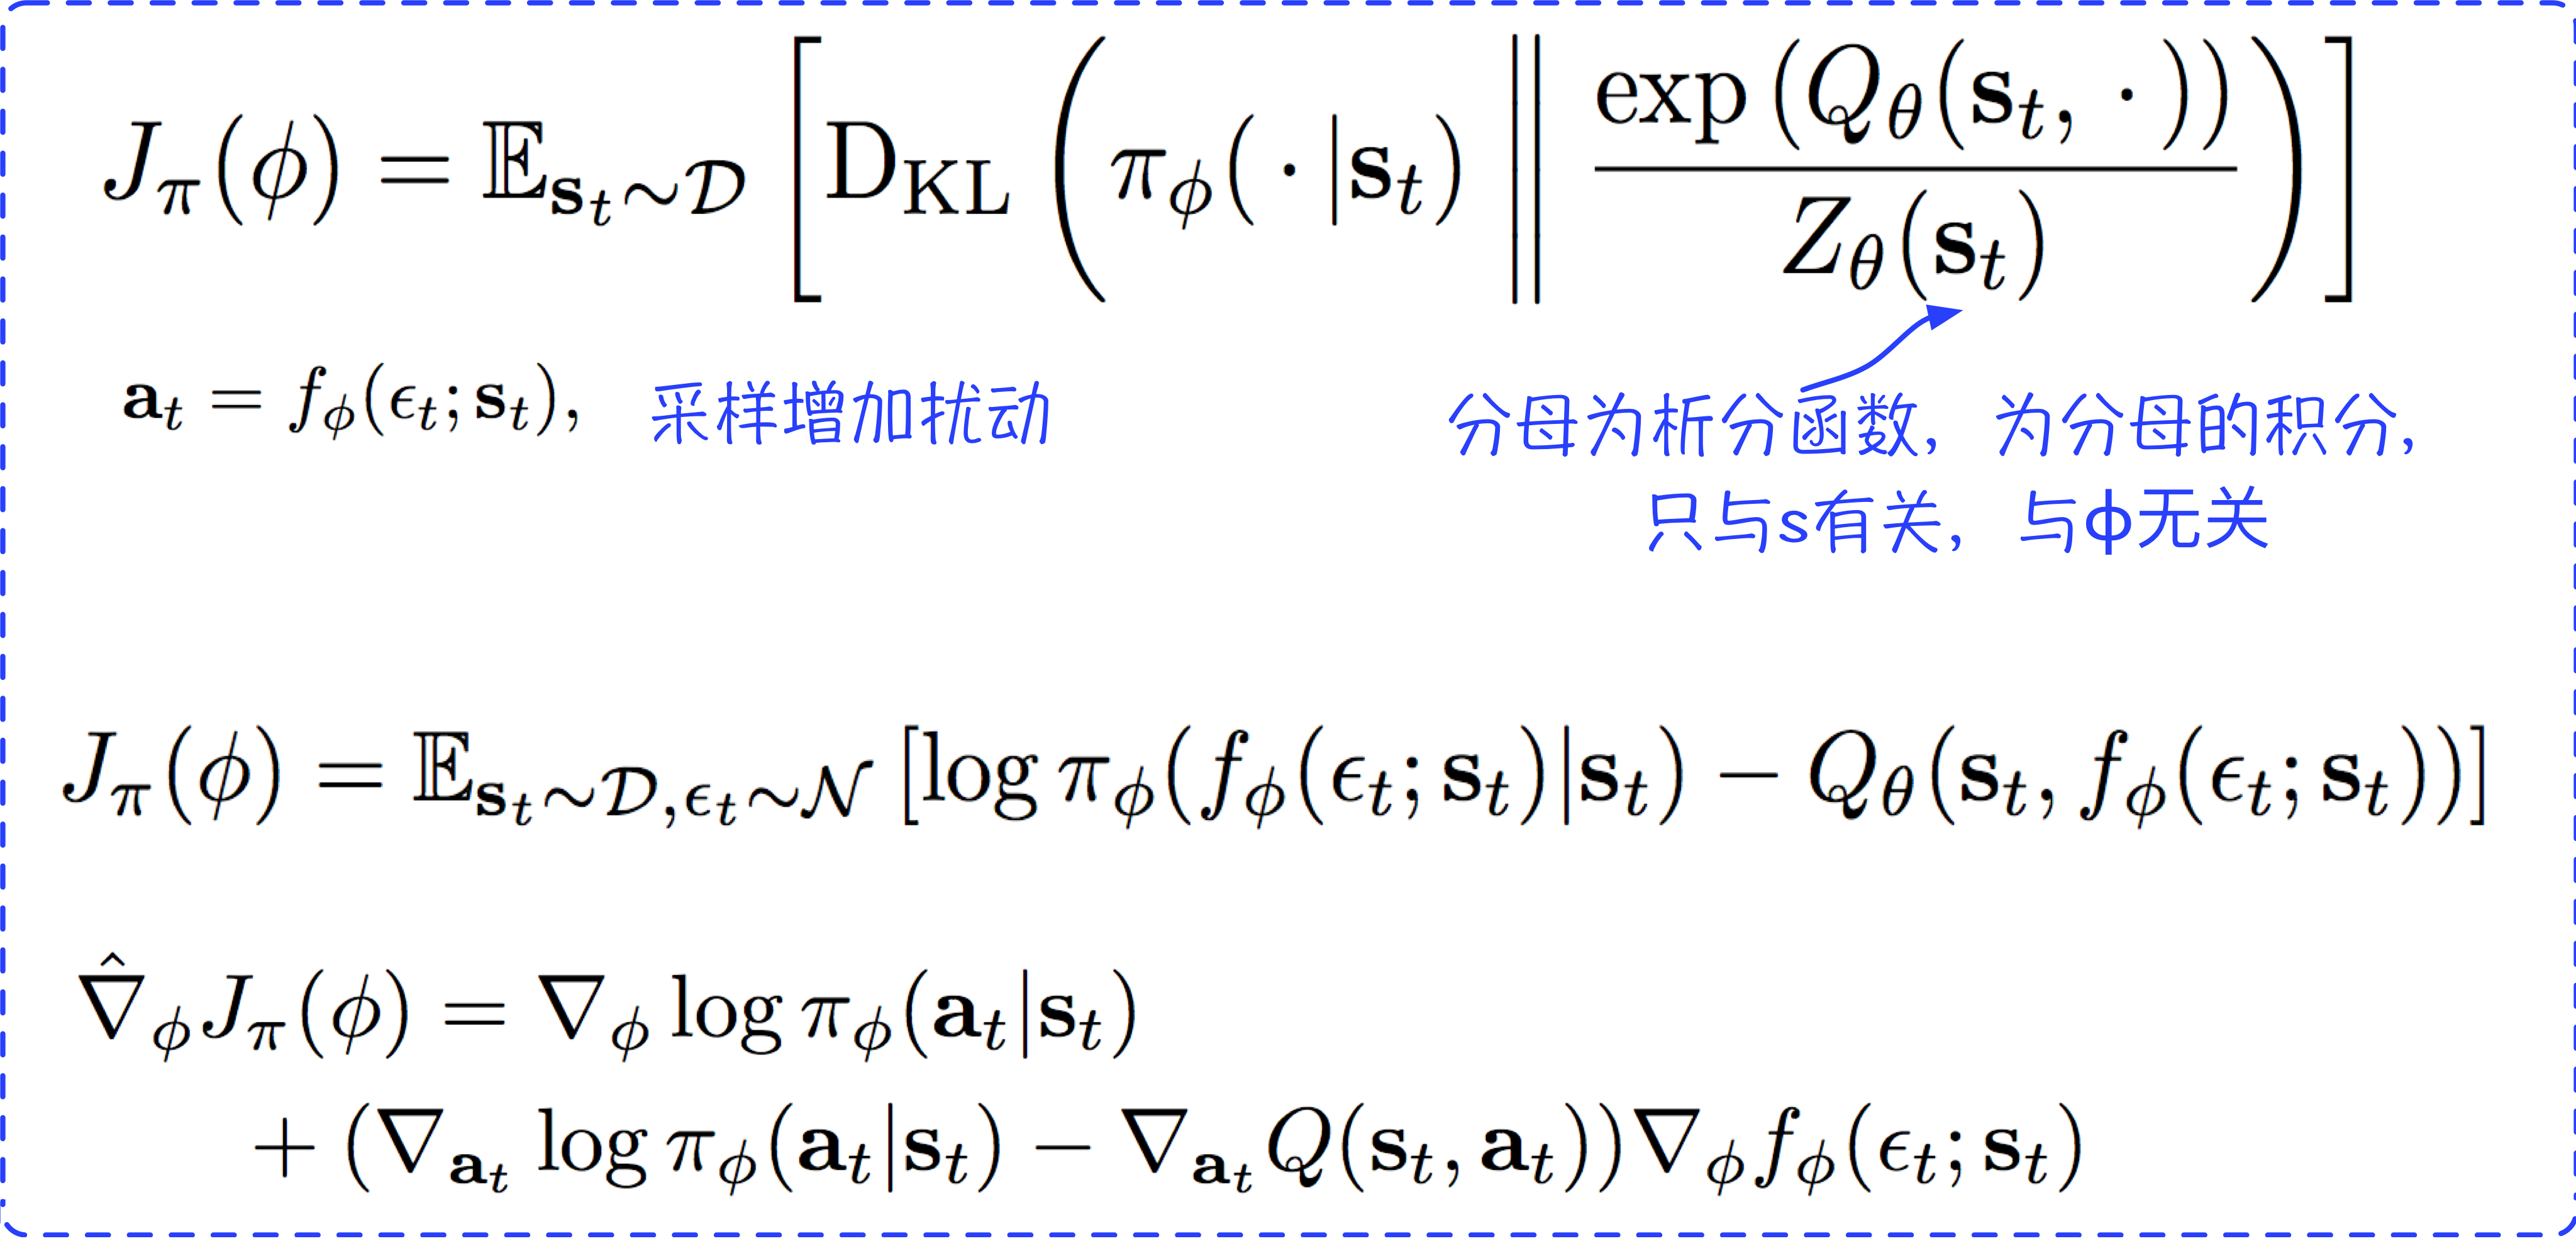
\includegraphics[scale=0.15]{pix/policy_objective.png}
\caption{Policy objective function}
%\label{fig:label}
\end{figure}


\subsection{学习过程}

整体采用Replay Buffer,三个目标函数分别进行梯度学习。

\begin{figure}[h]
\centering
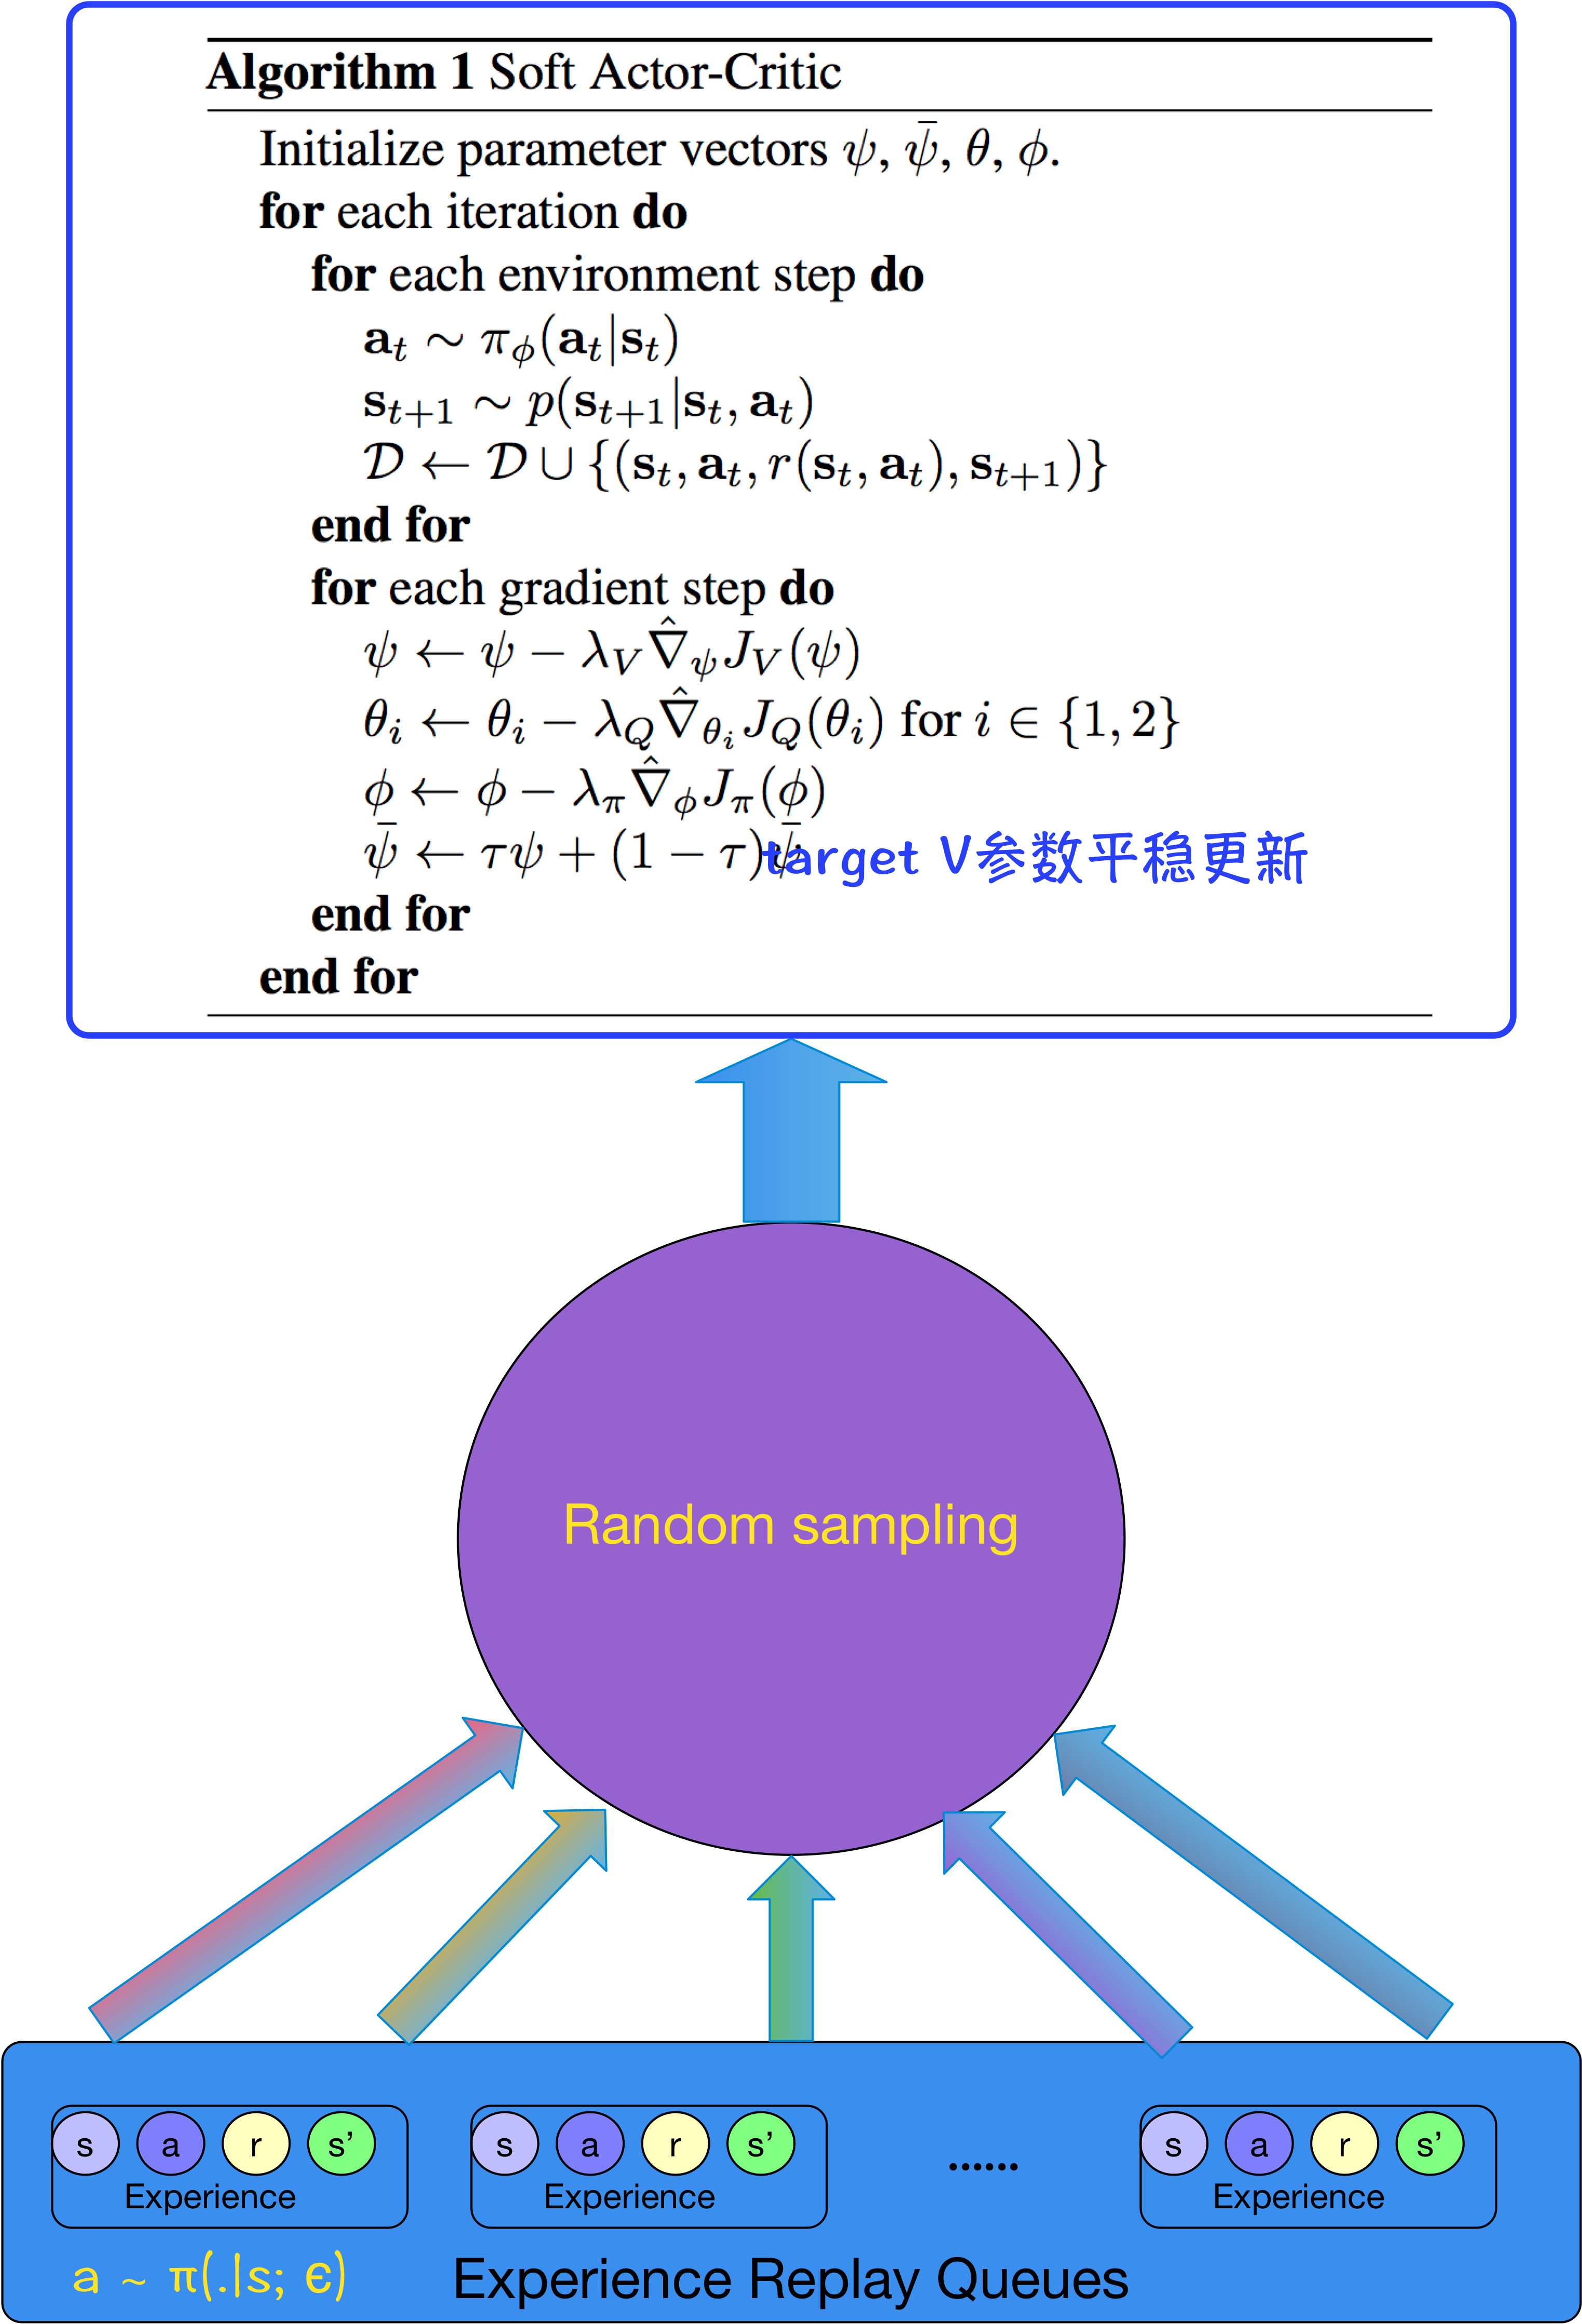
\includegraphics[scale=0.15]{pix/learning_process.png}
\caption{Learning process}
%\label{fig:label}
\end{figure}


\subsection{总结}

\begin{itemize}
%\setlength{\itemsep}{0pt}
%\setlength{\parsep}{0pt}
\setlength{\parskip}{0pt}
\item[1.]
SAC的关键是引入{\bf 最大熵},优化soft value。

\item[2.]
最大熵会使action{\bf 探索能力很强},模型效果更平稳,但注意需要场景也是接受较强的探索。

\item[3.]
从结构上讲,{\bf 模型冗余},在学习$\pi$和soft $Q$的情况下,又学习了soft $V$。

\item[4.]
由于面临的是连续动作空间,求期望的地方,采取了{\bf 采样近似},需要批次处理的数据集更加完整。

\item[5.]
优化技巧比较晦涩,感觉很难通用
\end{itemize}
